\documentclass[10pt,a4paper]{article}
\usepackage{blindtext}
\usepackage{subcaption}
\usepackage{graphicx}
\usepackage{tikz}
\usepackage{amssymb}
\usepackage{caption}
\usepackage{amsmath}
\usepackage{circuitikz}
\usepackage{hyperref}
\usepackage{amssymb}
\usepackage{amsmath}
\usepackage{listings}

\lstset{
    inputencoding=utf8,
    extendedchars=true,
    literate={á}{{\'a}}1 {é}{{\'e}}1 {í}{{\'i}}1 {ó}{{\'o}}1 {ú}{{\'u}}1 {ñ}{{\~n}}1 {Á}{{\'A}}1 {É}{{\'E}}1 {Í}{{\'I}}1 {Ó}{{\'O}}1 {Ú}{{\'U}}1 {Ñ}{{\~N}}1
}
\usepackage[spanish,activeacute,es-tabla]{babel}
\usepackage[utf8]{inputenc}
\usepackage{ifthen}
\usepackage{listings}
\usepackage{dsfont}
\usepackage{subcaption}
\usepackage{amsmath}
\usepackage[strict]{changepage}
\usepackage[top=1cm,bottom=2cm,left=1cm,right=1cm]{geometry}%
\usepackage{color}%
\newcommand{\tocarEspacios}{%
	\addtolength{\leftskip}{3em}%
	\setlength{\parindent}{0em}%
}

% Especificacion de procs

\newcommand{\In}{\textsf{in }}
\newcommand{\Out}{\textsf{out }}
\newcommand{\Inout}{\textsf{inout }}

\newcommand{\encabezadoDeProc}[4]{%
	% Ponemos la palabrita problema en tt
	%  \noindent%
	{\normalfont\bfseries\ttfamily proc}%
	% Ponemos el nombre del problema
	\ %
	{\normalfont\ttfamily #2}%
	\
	% Ponemos los parametros
	(#3)%
	\ifthenelse{\equal{#4}{}}{}{%
		% Por ultimo, va el tipo del resultado
		\ : #4}
}

\newenvironment{proc}[4][res]{%
	
	% El parametro 1 (opcional) es el nombre del resultado
	% El parametro 2 es el nombre del problema
	% El parametro 3 son los parametros
	% El parametro 4 es el tipo del resultado
	% Preambulo del ambiente problema
	% Tenemos que definir los comandos requiere, asegura, modifica y aux
	\newcommand{\requiere}[2][]{%
		{\normalfont\bfseries\ttfamily requiere}%
		\ifthenelse{\equal{##1}{}}{}{\ {\normalfont\ttfamily ##1} :}\ %
		\{\ensuremath{##2}\}%
		{\normalfont\bfseries\,\par}%
	}
	\newcommand{\asegura}[2][]{%
		{\normalfont\bfseries\ttfamily asegura}%
		\ifthenelse{\equal{##1}{}}{}{\ {\normalfont\ttfamily ##1} :}\
		\{\ensuremath{##2}\}%
		{\normalfont\bfseries\,\par}%
	}
	\renewcommand{\aux}[4]{%
		{\normalfont\bfseries\ttfamily aux\ }%
		{\normalfont\ttfamily ##1}%
		\ifthenelse{\equal{##2}{}}{}{\ (##2)}\ : ##3\, = \ensuremath{##4}%
		{\normalfont\bfseries\,;\par}%
	}
	\renewcommand{\pred}[3]{%
		{\normalfont\bfseries\ttfamily pred }%
		{\normalfont\ttfamily ##1}%
		\ifthenelse{\equal{##2}{}}{}{\ (##2) }%
		\{%
		\begin{adjustwidth}{+5em}{}
			\ensuremath{##3}
		\end{adjustwidth}
		\}%
		{\normalfont\bfseries\,\par}%
	}
	
	\newcommand{\res}{#1}
	\vspace{1ex}
	\noindent
	\encabezadoDeProc{#1}{#2}{#3}{#4}
	% Abrimos la llave
	\par%
	\tocarEspacios
}
{
	% Cerramos la llave
	\vspace{1ex}
}

\newcommand{\aux}[4]{%
	{\normalfont\bfseries\ttfamily\noindent aux\ }%
	{\normalfont\ttfamily #1}%
	\ifthenelse{\equal{#2}{}}{}{\ (#2)}\ : #3\, = \ensuremath{#4}%
	{\normalfont\bfseries\,;\par}%
}

\newcommand{\pred}[3]{%
	{\normalfont\bfseries\ttfamily\noindent pred }%
	{\normalfont\ttfamily #1}%
	\ifthenelse{\equal{#2}{}}{}{\ (#2) }%
	\{%
	\begin{adjustwidth}{+2em}{}
		\ensuremath{#3}
	\end{adjustwidth}
	\}%
	{\normalfont\bfseries\,\par}%
}

% Tipos

\newcommand{\nat}{\ensuremath{\mathds{N}}}
\newcommand{\ent}{\ensuremath{\mathds{Z}}}
\newcommand{\float}{\ensuremath{\mathds{R}}}
\newcommand{\bool}{\ensuremath{\mathsf{Bool}}}
\newcommand{\cha}{\ensuremath{\mathsf{Char}}}
\newcommand{\str}{\ensuremath{\mathsf{String}}}

% Logica

\newcommand{\True}{\ensuremath{\mathrm{true}}}
\newcommand{\False}{\ensuremath{\mathrm{false}}}
\newcommand{\Then}{\ensuremath{\rightarrow}}
\newcommand{\Iff}{\ensuremath{\leftrightarrow}}
\newcommand{\implica}{\ensuremath{\longrightarrow}}
\newcommand{\IfThenElse}[3]{\ensuremath{\mathsf{if}\ #1\ \mathsf{then}\ #2\ \mathsf{else}\ #3\ \mathsf{fi}}}
\newcommand{\yLuego}{\land _L}
\newcommand{\oLuego}{\lor _L}
\newcommand{\implicaLuego}{\implica _L}

\newcommand{\cuantificador}[5]{%
	\ensuremath{(#2 #3: #4)\ (%
		\ifthenelse{\equal{#1}{unalinea}}{
			#5
		}{
			$ % exiting math mode
			\begin{adjustwidth}{+2em}{}
				$#5$%
			\end{adjustwidth}%
			$ % entering math mode
		}
		)}
}

\newcommand{\existe}[4][]{%
	\cuantificador{#1}{\exists}{#2}{#3}{#4}
}
\newcommand{\paraTodo}[4][]{%
	\cuantificador{#1}{\forall}{#2}{#3}{#4}
}

%listas

\newcommand{\TLista}[1]{\ensuremath{seq \langle #1\rangle}}
\newcommand{\lvacia}{\ensuremath{[\ ]}}
\newcommand{\lv}{\ensuremath{[\ ]}}
\newcommand{\longitud}[1]{\ensuremath{|#1|}}
\newcommand{\cons}[1]{\ensuremath{\mathsf{addFirst}}(#1)}
\newcommand{\indice}[1]{\ensuremath{\mathsf{indice}}(#1)}
\newcommand{\conc}[1]{\ensuremath{\mathsf{concat}}(#1)}
\newcommand{\cab}[1]{\ensuremath{\mathsf{head}}(#1)}
\newcommand{\cola}[1]{\ensuremath{\mathsf{tail}}(#1)}
\newcommand{\sub}[1]{\ensuremath{\mathsf{subseq}}(#1)}
\newcommand{\en}[1]{\ensuremath{\mathsf{en}}(#1)}
\newcommand{\cuenta}[2]{\mathsf{cuenta}\ensuremath{(#1, #2)}}
\newcommand{\suma}[1]{\mathsf{suma}(#1)}
\newcommand{\twodots}{\ensuremath{\mathrm{..}}}
\newcommand{\masmas}{\ensuremath{++}}
\newcommand{\matriz}[1]{\TLista{\TLista{#1}}}
\newcommand{\seqchar}{\TLista{\cha}}

\renewcommand{\lstlistingname}{Código}
\lstset{% general command to set parameter(s)
	language=Java,
	morekeywords={endif, endwhile, skip},
	basewidth={0.47em,0.40em},
	columns=fixed, fontadjust, resetmargins, xrightmargin=5pt, xleftmargin=15pt,
	flexiblecolumns=false, tabsize=4, breaklines, breakatwhitespace=false, extendedchars=true,
	numbers=left, numberstyle=\tiny, stepnumber=1, numbersep=9pt,
	frame=l, framesep=3pt,
	captionpos=b,
}

\newcommand{\notimplies}{\;\not\!\!\!\implies}
\title{Paradigmas de Lenguajes de Programación}
\author{Tomás Agustín Hernández}
\date{}

\begin{document}
\maketitle

\begin{figure}[b]
    \centering
    \begin{tikzpicture}[remember picture,overlay]
        \node[anchor=south east, inner sep=0pt, xshift=-1cm, yshift=2cm] at (current page.south east) {
            \begin{minipage}[b]{0.5\textwidth}
                
\includegraphics[width=\linewidth]{logo_uba.jpg}
                \label{fig:bottom}
            \end{minipage}
        };
    \end{tikzpicture}
\end{figure}

\newpage
\section*{Programación Funcional}
Consiste en definir funciones y aplicarlas para procesar información. \\
Las funciones son verdaderamente funciones (parciales): 
\begin{itemize}
    \item Aplicar una función no tiene efectos secundarios.
    \item A una misma entrada le corresponde siempre la misma salida.
    \item Las estructuras de datos son inmutables.
\end{itemize}
Las funciones, además son datos como cualquier otro:
\begin{itemize}
    \item Se pueden pasar como parámetros.
    \item Se pueden devolver como resultados.
    \item Pueden formar parte de estructuras de datos. Ej.: Un árbol binario que en sus nodos hay funciones.
\end{itemize}
\subsection*{Expresiones}
Son secuencias de símbolos que sirven para representar datos, funciones, y funciones aplicadas a los datos. \\
Una expresión puede ser:
\begin{itemize}
    \item Un constructor: True, False, [], (:), 0, 1, 2. 
    \begin{itemize}
        \item Type Constructor: Es un constructor que se utiliza para crear un nuevo tipo.
        \item Data Constructor: Se utiliza para crear valores de ese tipo.
        \item Ej.: $data \ Color \ = \ Rojo \ | \ Verde \ | \ Azul$. Azul es un \textbf{data constructor} pues nos permite crear valores del tipo Color mientras que el Type Constructor es Color.
        \item Ej.: $data \ Complejo \ = \ C \ Float \ Float $. C es una función que recibe dos Float y es un constructor de Complejo.
    \end{itemize}
    \item Una variable: longitud, ordenar, x, xs (+), (*). 
    \item La aplicación de una expresión a otra: ordenar lista, not True, (+) 1. 
\end{itemize}
\subsection*{Función Parcialmente Aplicada}
Una función parcialmente aplicada es una función a las cuales se llama otra función pero no se le proporcionan todos los argumentos. \\
Ahora, es importante que para que esta función parcialmente aplicada tenga sentido se le manden todos los parámetros. \\
Es una especie de $ a \rightarrow b$
Ej.: 
\begin{lstlisting}
    add :: Int -> Int -> Int
    add x y = x + y

    add5 :: Int -> Int
    add5 = add 5

    add5 es una función que ejecuta la función parcial add pues le manda solo un parámetro y necesita dos.
   
\end{lstlisting}
Una buena pregunta entonces es ¿pero por qué es una función parcial add 5? Pues hay una función add5 que la implementa sin pasarle todos los parámetros directamente explícitamente.
\begin{lstlisting}
    add5 3 -> Este 3 llega como "y" a add

    add5 = add 5 
    add = 5 + y
    add = 5 + 3
    add = 8 

\end{lstlisting}

Otro ejemplo 
\begin{lstlisting}
    const :: a -> b -> a 
    const x y = x

    const (const 1) 2 -> const 1
    El llamado de (const 1) es una función parcialmente aplicada porque no envía el valor de y, sin embargo, const (const 1) 2 no la aplica parcialmente porque le termina mandando los dos parámetros.
\end{lstlisting}

\subsection*{Aplicación de Expresiones}
Es asociativa hacia la izquierda:
\begin{itemize}
    \item $ f \ x \ y \equiv \ (f \ x) \ y $
    \item $ ((((f \ a) \ b) \ c) \ d)$: Primero calcula el resultado que devuelve la expresión f enviando el valor de a. Nótese que la ídea seria que (f a) devuelva una expresión del tipo función pues luego le pasamos otro parámetro (b).
\end{itemize}
\subsection*{Importancia de la Aplicación de las Expresiones}
¿Qué sucede si aplicamos Head Tail l? Recordemos que la asociatividad a la izquierda haría algo así Head(Tail) l pero Tail en ese momento no es nada, y si aplicamos head explota. \\
En este caso los paréntesis son importantes: (head (tail l)) \\

Veamos otro ejemplo $map(\backslash x \rightarrow x \ 0) \ (map(+) \ [1, 2, 3])$. En este caso la asociatividad a la izquierda nos muestra algo así $map(\backslash x \rightarrow x \ 0) \ ((map(+) \ [1, 2, 3]))$ \\
Esto genera $map(\backslash x \rightarrow x \ 0) \ [2, 3, 4]$ ahora según lo que haga la función x, hace una cosa u otra. Imaginemos que lo llamamos como map (+1) [2, 3, 4] esto daría $[3, 4, 5]$
\section*{Función \$}
Aplica una función a un valor
\begin{lstlisting}
    g :: (a -> b) -> (a -> b)
    g x y = x y 
\end{lstlisting}
\subsection*{Construyendo una lista paso a paso con constructores}
Ej.: ¿Como construimos la lista [1, 2] utilizando constructores?
\begin{itemize}
    \item Lo primero que necesitamos, es un constructor de listas. Para eso tenemos la expresión (:). Recordando que la aplicación de expresiones es asociativo a izquierda.
    \item Veamos su tipo desde GHCI $(:) \ :: \ a \ -> \ [a] -> \ [a]$.
    \item Necesitamos enviarle un valor de tipo a, una lista y como resultado, la operación (:) devuelve una lista. 
    \item Preguntemos lo siguiente: ¿Con ((:) 1) nos basta para agregar a una lista? No, porque no estamos cumpliendo el tipado del constructor. Si quisieramos una lista con solamente el 1 si bastaría, pero acá también queremos el 2.
    \item Entonces, comenzamos aplicando la expresión (:) con el número 2, y ahí sí enviamos como segundo parámetro una lista vacía (que da como resultado) una lista vacía.
    \item (((:) 2) []) = [2]
    \item Por último, ((:) 1) [2] también cumple el tipo pues nos quedaría ((:) 1) [2] = [1, 2]
\end{itemize}
¿Y si quisieramos construir 1, 2, 3, 4? Recordemos la asociatividad a la izquierda, pero a la hora de querer utilizar una expresión, hay que cumplir el tipado. Hasta que ese tipado no se cumpla, Haskell tratará de resolver la expresión más profunda para ver si reduciendo cumple el tipo. \\
\[((:) 1) \ (((:) \ 4)(((:) \ 2) (((:) \ 3) \ [])))\] \\
Esto lo podemos ver como $a \rightarrow (b \rightarrow (c \rightarrow (d))) $ pues para conocer a, necesitamos construir la lista de la derecha, para conocer a b necesitamos la lista de la derecha, para conocer a c necesitamos la lista de d, y d inicializa la lista vacía. Esto es importantísimo porque claramente no podríamos usar (:) 1 sin una lista. Entonces Haskell evalúa todo lo de la derecha hasta que obtenga una lista. Si no se obtuviera una lista, sería inválido.
\section*{Polimorfismo}
Sucede en aquellas expresiones que tienen más de un tipo. 
\begin{itemize}
    \item $ id \ :: \ a \rightarrow a $
    \item $(:) :: a \rightarrow [a] \rightarrow [a]$
    \item $fst :: (a, b) \rightarrow a$
    \item $cargarStringArray :: String -> [] \rightarrow [String]$. No es una expresión Polimórfica.
\end{itemize}
\textbf{Nota}: Es importante que si tenemos 2 parámetros de tipo a significa que los dos parámetros deben ser de ese tipo. Si tenemos 2 parámetros uno de tipo a y uno de b podría suceder que sean diferentes pero puede que sean el mismo. 
\textbf{Importante}: Recordar que si usamos operadores, colocar las clases que correspondan. Ej.: $a>0$ a debe ser $(Num a, Ord a)$. \\
Véase \hyperref[subsec:clases_tipos]{\underline{\textbf{anexo}}} para ver ejemplos de las clases de tipos.
\section*{Polimorfismo con Clases (Type Classes)}
Es posible limitar el polimorfismo a clases específicas. Es decir, si nos mandan un tipo $a$ podemos decir que ese tipo $a$ es genérico pero de una clase específica. \\
Ejemplo: $func :: Num \ a \implies a \rightarrow a \rightarrow a$ \\
En este caso, $Num \ a $ es una Type Class.
\section*{Modelo de Cómputo (cálculo de valores)}
Dada una expresión, se computa su valor usando las ecuaciones siempre y cuando estén bien tipadas. \\
\textbf{Importante}: Que una expresión se cumpla el tipado, no significa que devuelva un valor.
\begin{itemize}
    \item $sumarUno :: a -> a$: No falla nunca.
    \item $division :: a -> b$: Falla si b = 0. Esto nos demuestra que aunque los parámetros estén bien tipados, podemos tener indefiniciones.
\end{itemize}
\subsection*{¿Cómo está dado un programa en Funcional?}
Un programa funcional está dado por un conjunto de \textbf{ecuaciones orientadas}. Se les llama de esta forma pues del \textbf{lado izquierdo está lo que define y del lado derecho la definición} (o expresión que produce el valor)
Una ecuación e1 = e2 se interpreta desde dos puntos de vista
\begin{itemize}
    \item \textbf{Denotacional}: Declara que e1 y e2 tienen el mismo significado. 
    \begin{itemize}
        \item "\textbf{Denotan} lo mismo"
    \end{itemize}
    \item \textbf{Operacional}: Computar el valor de e1 se reduce a computar el valor de e2.
    \begin{itemize}
        \item "\textbf{Operan} de la misma forma"
    \end{itemize}
\end{itemize}
\subsection*{¿Cómo es el lado izquierdo de una ecuación orientada?}
No es una expresión arbitraria. Debe ser una función aplicada a \textbf{patrones}. \\
Un patrón puede ser: 
\begin{itemize}
    \item Una variable: a, b, c.
    \item Un comodin: \textunderscore. 
    \item Un constructor aplicado a patrones: Recordemos que un constructor sería algo que construye un tipo. 
    \begin{itemize}
        \item True, False, 1, etc.
    \end{itemize}
\end{itemize}
\textbf{Importante}: El lado izquierdo NO debe contener variables repetidas. \\
Ej.: $iguales \ x \ x \ = \ True$ es una expresión mal formada. Esto pues dos valores que pueden ser diferentes, no pueden caer en la misma variable. \\
Ej.: $predecesor \ (n+1) \ = \ n$ también está mal formada porque estamos haciendo un cálculo del lado izquierdo, y recordemos que del lado izquierdo solo hay definiciones. Del lado derecho se hacen los cómputos o cálculo de los valores.
\subsection*{¿Cómo evalúamos las expresiones?}
\begin{itemize}
    \item Buscamos la subexpresión más externa que coincida con el lado izquierdo de una ecuación.
    \item Reemplazar la subexpresión que coincide con el lado izquierdo de la ecuación por la expresión correspondiente al lado derecho.
    \item Continuar evaluando la expresión resultante.
\end{itemize}
\subsection*{¿Cuando se detiene la evaluación de una expresión?}
\begin{itemize}
    \item Cuando el programa estalla.
    \begin{itemize}
        \item Loop infinito.
        \item Indefinición.
    \end{itemize}
    \item Cuando la expresión es una función \textbf{parcialmente aplicada}. ¿que seria esto? ¿se refiere a utilizar mal la función parcialmente aplicada? 
    \item La expresión es un constructor o un constructor aplicado. Ej.: True, (:) 1, [1, 2, 3]. 
    \begin{itemize}
        \item Yo lo veo como algo más del tipo: una fórmula atómica o algo irreducible.
    \end{itemize}
\end{itemize}
\subsection*{¿Cómo ayuda el Lazy Evaluation (Evaluación Perezosa) a Haskell?}
Muchas veces nos ayuda a evitar tocar con un valor indefinido aunque esté ahí. Como no evalúa cosas que no necesita, si hay un indefinido por ahí y no necesita ni siquiera llegar, no lo toca.
\begin{lstlisting}
    indefinido :: Int 
    indefinido = indefinido 
    head(tail [indefinido, 1, indefinido])
\end{lstlisting}
¿Qué hace tail? Toma la cola de la lista, entonces como resultado arroja [1, indefinido] (ni siquiera evaluó el primer indefinido) \\ 
¿Qué hace head ahora entonces? [1] (ni siquiera evaluó el indefinido del final)
\subsection*{Importancia del orden de las Ecuaciones}
El criterio más fuerte debe ir por encima del resto. Porque puede haber un caso que matchee y nunca se evalúe el siguiente caso. \\
Veamos un ejemplo: 
\begin{lstlisting}
    esCorta (_:_:_) = False
    esCorta _ = True 
\end{lstlisting}

Considerando este orden: 
\begin{itemize}
    \item Si mando una lista que siempre tiene $\ge$ 3 elementos da False.
    \item Si mando una lista que tiene $ < $ 3 elementos es siempre True.
\end{itemize}

Cambiemos el orden y veamos qué cambia
\begin{lstlisting}
    esCorta _ = True 
    esCorta (_:_:_) = False
\end{lstlisting}
Considerando este orden: 
\begin{itemize}
    \item Si la lista tiene 0, 1, 2, 3, 4, ... n elementos siempre dará True.
\end{itemize}
En la segunda aplicación ¡nunca caemos en el caso 2! y esto es importante porque sabemos que si tiene 1 cae siempre en la primera.
\section*{Notación Infija \& Notación Prefija}
\textbf{Infija}: argumento + funcion + argumento \\
\textbf{Prefija}: funcion + argumentos \\
\textbf{Importante}: $(\le) 18 \neq (\le 18)$ pues la opción de $(\le) 18$ sería $(18 \le x)$ mientras que $(\le 18)$ sería $(x \le 18)$. Donde claramente denota que el parámetro cuando está fuera de la notación infija es el primer argumento mientras que si lo ponemos adentro hardcodeamos su posición. Es decir $(18 \le)$ estaríamos diciendo $(18 \le x)$
\section*{Currificación}
Una función es currificada cuando tiene la siguiente forma $ ab :: Int -> Int -> Int $ \\
Esto puede parecer que recibe 2 parámetros y devuelve uno, pero en realidad lo que hace es básicamente por cada parámetro asociar a la izquierda y hacer una función por cada parámetro. \\
Es decir, sería algo así $ab::Int -> (Int -> Int)$ \\
La función Curry \textbf{NO CAMBIA} la manera en que la función original currificada recibe los argumentos, sino que, la función curry es una especie de $puente$ para que nosotros mandemos los argumentos separados y los aplique a la función no currificada. \\
\textbf{Importante}: No tiene sentido hablar de currificación cuando las funciones tienen un solo parámetro \\
Las funciones currificadas son realmente importantes en la Programación Funcional porque nos permite aplicarlas de forma parcial. Es una especie mas reutilizable. \\

Una función no currificada tiene esta pinta $suma::(Int, Int) -> Int -> Int$ porque acá estoy obligando a la función suma a recibir una tupla de elementos, no puedo ir mandando de a uno parcialmente. \\
Véase \hyperref[subsec:curry_uncurry]{\textbf{anexo}} para armar una función curry y uncurry
\section*{Funciones de Orden Superior}
Son funciones que reciben como parámetro otras funciones. 

Definamos la composición de funciones $(g \ .\ f)$ \\
Recordemos que en Álgebra vimos Composición de Funciones y es algo así: sean $A:B \rightarrow C$ y $D:A \rightarrow B$ \\

La composición gof es $A \rightarrow B$. Es decir, va desde el dominio de D hasta la imagen de A. (la salida de una función debe ser la entrada de la otra.) \\

En Haskell, la podemos definir así
\begin{lstlisting}
    ent: Entrada sal: Salida

    (.) :: (b -> c) -> (a -> b) -> (a -> c)
    
    Queremos: (g . f) x => g (f x) 

    Desglosemos
    (.) :: (ent. de g -> sal. de g) -> (ent. de f -> sal. de f) -> (ent. de f -> sal. de g)
    
    El resultado de la composición nos da una nueva función que tiene como entrada un valor de tipo a, y la salida es un valor de tipo c.
    
    Entonces, primero se evalúa f x, lo cual produce un resultado de tipo b.
    
    Luego, este resultado (de tipo b) se pasa a g, produciendo un resultado de tipo c.
  
    (g . f) x: envía el parámetro x a la función f, y el resultado de f x se manda a g. Esto da como resultado g (f x)
\end{lstlisting}
Otra forma de definir la composición es usando Notación Lambda.
\begin{lstlisting}
    (.) :: (b -> c) -> (a -> b) -> (a -> c)
    g . f = \ x -> g (f x)
\end{lstlisting}
Recordemos que esto es algo recordable pues $fog$ seria meter g adentro de f y para eso, la salida de g debe ser la entrada de f. Y luego se devuelve como salida el dominio de g y la salida de f.
Nótese que la notación lambda es súper útil para definir funciones sin nombre, que solamente hagan algo. Esto es muy útil cuando queremos mandar una función por parámetro y que una función dada la llame a esta función.
\subsection*{Llamados estándar vs llamados en composición}
$not(null x) \equiv (not . null) x$ \\
Esto quiere decir que si primero componemos todas las funciones que queremos aplicarle a un valor, es lo mismo que ir aplicando de una a una las funciones al argumento.
\textbf{Importante}: La composición funciona \textbf{sí y solo sí} alguna de las funciones está parcialmente aplicada. Ej.: $(== 0) . mod n m$ no funciona, pero $(== 0) . mod n$ sí.
\subsection*{Funciones Lambda}
Son funciones anónimas, es decir, no tienen nombre.  \\
\textbf{($\backslash x \rightarrow x+1$)}: Es una función anónima que dado un x, te devuelve una función que le aplica x+1.
\subsection*{Funciones Lambda Anidadas}
$\backslash y \rightarrow (\backslash x \rightarrow y)$: Esto a ojo es una función constante, porque dado un valor y, se aplica la función x pero se devuelve el mismo valor y. \\
Los parámetros se obvían en algunos casos, este es uno. La mejor forma sería $\backslash y \rightarrow \backslash x \rightarrow y$. \\
Mejor notación para funciones anidadas: $\backslash y \ x \rightarrow y$
\subsection*{Reducción de Lambda}
Preguntar $foldr(\backslash x \ rec \rightarrow fx:rec) \equiv \backslash x \rightarrow (:)(fx)$ y $ \backslash x \rightarrow ex \equiv e$
\section*{Asignar nombre a una función}
$a = \backslash x \rightarrow x $: al nombre \textbf{a} le asigno la función anónima $\backslash x \rightarrow x$
\subsection*{¿Para qué queremos funciones de orden superior? Pt 1}
\begin{lstlisting}
    dobleL :: [Float] -> [Float]
    dobleL [] = []
    dobleL (x:xs) = x * 2 : dobleL xs 

    esParL :: [Int] -> [Bool]
    esParL [] = []
    esParL (x:xs) = x 'mod' 2 == 0 : esParL xs
\end{lstlisting}

¿Qué es lo que tienen en común? Todas tienen una estructura bastante similar.
\begin{lstlisting}
    g [] = []
    g (x : xs) = f x : g xs
\end{lstlisting}
Lo único que cambia es \textbf{qué se hace} en cada paso recursivo. \\
Hagamos una pregunta ¿la cantidad de elementos de la entrada es igual a la de la salida? en este caso sí pero ¿qué operación se está haciendo? se están haciendo ciertas manipulaciones de los datos y se devuelve la información modificada en una lista nueva. \\
Esto, en varios lenguajes se conoce como \textbf{map}. Se hace una manipulación de los datos pero se devuelve \textbf{la misma cantidad de elementos}. 
\subsection*{Map}
Recibe como parámetro una función que es aplicada a todos los elementos y devuelve una lista nueva. Se utiliza para modificar los valores de una lista dada según lo que haga la función. \\
\begin{lstlisting}
    map :: (a -> b) -> [a] -> [b]
    map f [] = []
    map f (x : xs) = f x : map f xs 
\end{lstlisting}

Entonces, podemos definir \textbf{qué operación de modificación} se le realizan a los elementos de una lista dada.
\begin{lstlisting}
    multiplicarPorDos :: [a] -> [b]
    multiplicarPorDos xs = map (\x -> x * 2) xs 

    dividirPorDos :: [a] -> [b]
    dividirPorDos xs :: map(\x -> x / 2) xs 
\end{lstlisting}
Entonces gracias a Map nos abstraemos de tener miles de funciones con la misma estructura pero solo cambien \textbf{qué hacen} con los elementos. 
\subsection*{¿Para qué queremos funciones de orden superior? Pt 2}
\begin{lstlisting}
    negativos :: [Int] -> [Int]
    negativos [] = []
    negativos (x:xs) = if x < 0 
                       then x : negativos xs
                       else negativos xs 
    
    pares :: [Int] -> [Int]
    pares [] = []
    pares (x:xs) = if x 'mod' 2 == 0
                   then x : pares xs 
                   else pares xs
\end{lstlisting}
¿Qué es lo que tienen en común? Todas tienen una estructura bastante similar, pero lo único que cambia es \textbf{cuando vamos a agregar a la lista los elementos}. \\

\begin{lstlisting}
    g [] = []
    g (x:xs) = f x : g xs
\end{lstlisting}

Hagamos una pregunta ¿la cantidad de elementos de la entrada es igual a la de la salida? Puede que sí, puede que no.   \\
¿Qué operación se está haciendo? se están filtrando ciertos elementos de una lista que no cumplan una condición dada. \\
Esto, en varios lenguajes se conoce como \textbf{filter}. Se devuelve una nueva lista con los elementos que cumplan una condición dada.
\subsection*{Filter}
Recibe como parámetro una función que es aplicada a todos los elementos. Se utiliza para "borrar" elementos de una lista, o quitar aquellos que no cumplan un criterio dado. 
\begin{lstlisting}
    filter :: (a -> Bool) -> [a] -> [b]
    filter p [] = []
    filter p (x : xs) = if p x
                        then x : filter p xs 
                        else filter p xs
\end{lstlisting}

La función que le envíamos es para especificar \textbf{qué elementos nos queremos quedar}.

Entonces, podemos definir \textbf{qué operación de filtro} se le realizan a los elementos de una lista dada.
\begin{lstlisting}
    eliminarImpares :: [a] -> [b]
    eliminarImpares xs = filter (\x -> x `mod` 2 == 0) xs 

    borrarNegativos :: [a] -> [b]
    borrarNegativos xs = filter(\x -> x > 0) xs 
\end{lstlisting}
Entonces gracias a Filter nos abstraemos de tener miles de funciones con la misma estructura pero solo cambien \textbf{con qué elementos nos quedamos} dada una condición
\section*{Recursión}
¿Qué tienen en común los siguientes problemas? ¿En qué difieren? 
\begin{lstlisting}
    concat :: [[a]] -> [a]
    concat [] = []
    concat (x:xs) = x ++ concat xs

    reverso :: [a] -> [a]
    reverso [] = []
    reverso (x:xs) = reverso xs ++ [x]

    sum :: [int] -> int 
    sum [] = 0
    sum (x:xs) = x + sum xs

    En común: 
        1. Todos tienen un caso base, pero es diferente.
        2. Todos hacen un paso recursivo, pero cambia la operación que hacen. 
        3. El tipo de entrada puede no coincidir con el de la salida.
\end{lstlisting}
En este tipo de problemas lo mejor que podemos hacer es realizar una especie de función que nos permita modularizar lo más posible y aquello que difiere, pasarlo por parámetros. \\
Este tipo de problemas lo podemos solucionar con Foldr. 
\subsection*{Recursión Estructural (foldr)}
\begin{itemize}
    \item Se trabaja solamente con la cabeza de la lista.
    \item Se hace recursión sobre la cola pero no se tiene acceso a ella, sino al llamado recursivo. 
    \item La recursión es la clásica, va desde derecha a izquierda. La R de foldr es de Right. 
\end{itemize}
Su estructura formal es la siguiente 
\begin{lstlisting}
    g [] = <caso base> -> valor 
    g (x:xs) = <caso recursivo> -> función cabeza de la lista y resultado de la recursión.
\end{lstlisting}
Por lo tanto foldr se define como
\begin{lstlisting}
    foldr :: (a -> (b -> b)) -> b -> [a] -> b 
    foldr f z [] = <
    foldr f z (x:xs) = f x (foldr f z xs)
\end{lstlisting}
¿Qué es lo que produce foldr (:) []? Es una identidad sobre listas porque haría recursión sobre una lista vacía. \\
¿Qué es lo que hace la siguiente función foldr? $ foldr(\backslash x \ r \rightarrow x) \ 0 \ [1, 2]$ 
\begin{itemize}
    \item Toma la lista y hace recursión. Empieza con el 2, ejecuta la función y devuelve 2. Hace el paso recursivo.
    \item Toma la lista y hace recursión. Ahora sigue con el 1, recibe 1 y la salida es 1. 
    \item Esta función agarra el primer elemento de una lista, sería el head.
\end{itemize}
\textbf{Importante}: Foldr puede trabajar con listas infinitas. \\
Véase \hyperref[subsec:folder_ex]{anexo} para ver ejemplos de Foldr. 
\subsection*{Iteración (foldl)}
Este tipo de recursión es más que recursión una iteración, en este caso empezamos yendo desde el primer valor hasta el último. \\
En este enfoque voy modificando una solución parcial. \\
Por lo tanto foldl se define como
\begin{lstlisting}
    foldl :: (b -> a -> b) -> b -> [a] -> b 
    foldl f ac [] = ac
    foldl f ac (x:xs) = foldl f (f ac x) xs
\end{lstlisting}
¿Qué es lo que sucede en el siguiente ejemplo? \\
\begin{lstlisting}
    foldl (\x y -> 1) 0 unos
    foldl f (f 0 1) unos
    foldl f(f(f 0 1) 1) unos
\end{lstlisting}
Esto es in-realizable con foldl. Es decir, foldl no puede manejar listas infinitas.
\subsection*{¿Por qué foldl es peor que foldr?}
\textbf{foldl}: Procesa la lista de izquierda a derecha, lo que requiere evaluar toda la lista antes de devolver un resultado, lo que no es posible con listas infinitas. \\
\textbf{foldr}: Procesa la lista de derecha a izquierda, permite trabajar de manera perezosa y puede manejar listas infinitas si la función y el valor inicial permiten una evaluación parcial o completa sin necesidad de procesar todos los elementos.
\subsection*{Recursión Primitiva (recr)}
No existe en Haskell. Es una manera de nosotros podemos tener las mismas ventajas de foldr pero en este caso, la recursión primitiva nos permite utilizar la cola de la lista 
\begin{itemize}
    \item Se trabaja solamente con la cabeza de la lista y la cola.
    \item Se hace recursión sobre la cola.
\end{itemize}
Su estructura forma les la siguiente 
\begin{lstlisting}
    g [] = b
    g (x:xs) = f x xs (g xs)
\end{lstlisting}
Por lo tanto recr se define como 
\begin{lstlisting}
    recr :: (a -> [a] -> b ->b) -> b -> [a] -> b 
    recr f z [] = z
    recr f z (x:xs) = f x xs (recr f z xs)
\end{lstlisting}
\section*{Tipos}
Existen diferentes maneras de definir tipos. Esto es según sea el objetivo.
Definimos tipos con la palabra \textbf{data} + Nombre = Tipo1 | Tipo2 | Tipo 3 \\
Si hacemos en GHCI $:t Tipo1$ saldrá que es de tipo Nombre. \\
\textbf{Nota}: $|$ indica que a continuación hay otro tipo.
\subsection*{Tipos Comunes}
Son no recursivos, ej: $data Dia = Lu | Ma | Mi | Mie | Ju | Vi | Sa | Do $ \\
Lu, Ma, Mi, ... son constructores del tipo dia. \\
Los argumentos podrán ser recibidos diciendo qué tipo se espera, y usamos pattern matching para utilizarlos.
\begin{lstlisting}
    EsLunes :: Dia -> Bool
    EsLunes Lu = True 
    EsLunes _ = False 

    EsFinDeSemana :: Dia -> Bool
    EsFinDeSemana Sa = True 
    EsFinDeSemana Do = True 
    EsFinDeSemana _ = False 
\end{lstlisting}
\subsection*{Tipos con Funciones}
Los tipos también pueden tener tipos que necesiten argumentos. Difieren en la info que devuelven. \\
Ej.: data Persona = LaPersona String String Int \\
\textbf{Importante}
\begin{itemize}
    \item Si evaluamos $:t LaPersona$ sin enviar los argumentos retornará $LaPersona :: String -> String -> Int$. 
    \item Si evaluamos $:t LaPersona "T", "H", 23$ enviando los argumentos retornará que LaPersona es de tipo Persona
\end{itemize}
\begin{lstlisting}
    Edad :: Persona -> Int 
    Edad (LaPersona n a e) = e

    Cumpleaños :: Persona -> Persona 
    Cumpleaños (LaPersona n a e) = LaPersona n a (e+1)
\end{lstlisting}
\textbf{Importante}: Nótese que estamos devolviendo \textbf{una nueva persona}. En programación funcional no existe el concepto de "modificar" algo, sino crear algo nuevo con lo anterior y cambiarle algo.
\subsection*{Tipos Recursivos}
Cuando tengo tipos recursivos, las funciones que los usen deben manejar casos bases y la recursión \\
Ej.: data Nat = Zero | Succ Nat 
\subsection*{Tipos Polimórficos} 
Al igual que las funciones, podemos definir que los tipos tengan constructores de un tipo específico.
\begin{lstlisting}
    data List a = Vacia | Const a (List a)
\end{lstlisting}
\subsection*{Importante en Tipos}
No se puede repetir un mismo constructor para un mismo tipo. \\
Es decir
\begin{lstlisting}
    data List = Vacia | Cons Int ListI 
    data List a = Vacia | Cost a (List a)

    Error. No puede estar Vacia como constructor de dos tipos diferentes.
\end{lstlisting}
\section*{Listas}
\begin{itemize}
    \item Por extensión: Es dar la lista implícita escribiendo todos sus elementos. Ej. [1, 2, 3]
    \item Secuencias: Progresiones aritméticas en un rango particular. Ej.: [3..7] es la lista que tiene los números del 3 al 7.
    \item Por compresión: Se definen de la siguiente manera [expresion | selectores, condiciones]. Ej.: [(x,y) | x <- [0..5], y <- [0..3], x+y==4] es la lista de pares que tienen elementos de x e y que dan menos que 4
\end{itemize}
\section*{Lista Infinitas}

\section*{Recordando Haskell}
Para ejecutar un archivo hay que instalar GHCI. Una vez instalado, nos paramos en la terminal en el directorio donde está el archivo que queremos ejecutar. 
\begin{itemize}
    \item Cargar archivo: :l nombreArchivo
    \item Ver tipo: :type tipo 
    \item Ejecutar funcion: funcion parametro1 parametro2...
    \item Recargar archivo: :r
    \item Si necesitamos hacer cálculos para mandar un parámetro, usar paréntesis: Ej.: otherwise = n * factorial(n-1)
\end{itemize} 
\section*{Maybe}
El Maybe se utiliza en Haskell para recibir/devolver respuestas condicionales que pueden ser de un tipo u otro. \\

Se define como $data \ Maybe \ a \ = \ Nothing \ | \ Just \ a$ \\

Ej.: $ devolverFalsoSiVerdadero \:: \ Bool \rightarrow Prelude.Maybe \ Bool $ \\

El Maybe deja la puerta abierta a un valor posible "Nothing". Entonces tenemos dos casos: Si me envian un True devuelvo False (tipo bool), caso contrario, devuelvo Nothing. 

\section*{Either}
El Either se utiliza en Haskell para poder recibir/devolver un parámetro que podría ser de un tipo u otro. \\
Se define como $ data \ Either \ a \ b \ = \ Left \ a \ | \ Right \ b $ \\

Para poder saber qué operación hacer según el tipo literalmente en código usamos (Left valor) o (Right valor). \\

Ej.: $ devolverRepresentacionIntBool \ :: \ Either \ Int \ Bool \ \rightarrow \ Int $ \\

Si es un entero, devuelvo ese mismo entero porque no hago nada. Eso lo hacemos con $Left(a) \ = \ a$, ahora, si el tipo es booleano tengo que decir explícitamente la respuesta según su valor. Es decir, $Right(False) \ = \ 0$ sino, $Right(True) \ = \ 1$.

\section*{Declaración de tipos en Haskell}
Se utiliza $data \ nombretipo \ tipo \ = \ Tipo \ 1 \ | \ Tipo \ 2$ 
El $|$ se interpreta como \textbf{o bien}
\section*{Árboles Binarios}
Es un tipo (para mi parecer) meramente recursivo. \\
$data \ AB \ a \ = \ Nil \ | \ Bin \ (AB \ a) \ a \ (AB \ a)$
Nótese que es algo re contra recursivo, porque para definir el tipo de AB a decimos que es un Bin que a su vez es de AB a y a su vez AB a es otro árbol binario. \
Veamos unos ejemplos de esto
\begin{itemize}
    \item Bin (Nil) Nil (Nil): es el árbol que no tiene ni siquiera raíz. Y nótese que en cada paréntesis es importante indicar el Nil pues es la forma de que el tipado de Haskell nos lo acepte.
    \item Bin (Bin Nil 3 Nil) 4 (Bin Nil 6 Nil): Es el árbol que comienza con un Nodo raíz que tiene el valor de 4. El hijo izquierdo del Nodo con valor 4 es otro árbol binario que tiene como valor 3 en su nodo y no tiene hijos. El hijo derecho del Nodo con valor 4 es otro árbol binario que tiene como valor 6 en su Nodo y no tiene hijos. 
\end{itemize}
Y así sucesivamente, veamos un dibujo para tener algo más visual. \\
El siguiente árbol binario: Bin (Bin (Bin Nil 2 Nil) 3 Nil) 4 (Bin (Bin Nil 5 Nil) 6 Nil) representa el siguiente:
\[\begin{minipage}[b]{0.5\textwidth}
    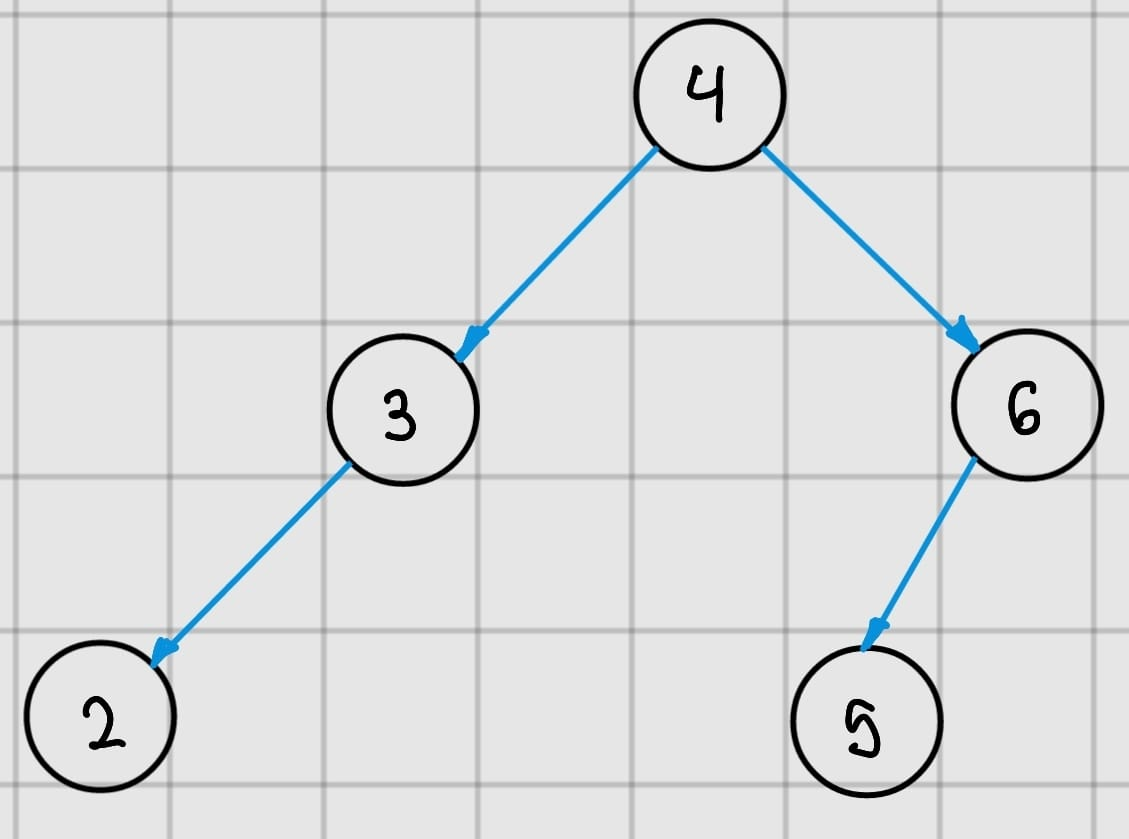
\includegraphics[width=\linewidth]{assets/abb_haskell.jpg}
\end{minipage}\]
\subsection*{Curry \& Uncurry}
\label{subsec:curry_uncurry}
Digamos que necesitamos currificar una función que recibe una tupla de elementos. Es decir, algo así: $ suma :: (Int, Int) -> Int $ \\
Por la definición de curry necesitamos que por cada argumento, haya una función que lo devuelva, por lo tanto el resultado sería algo así $ suma :: Int -> Int -> Int $. \\
Veamos el tipo de función que queremos currificar: $((a, b) -> c)$, esto lo queremos llevar a $a -> b -> c$. \\
Por lo tanto nuestra función curry sería algo así: 
\begin{lstlisting}
    curryOwn :: ((a, b) -> c) -> a -> b -> c
    curryOwn f a b = f (a, b) 
\end{lstlisting}
Entonces, digamos que queremos hacer la suma currificada. 
\begin{lstlisting}
    sumTuple :: (Float, Float) -> Float
    sumTuple (x, y) = x + y

    sumarCurry :: Float -> Float -> Float
    sumarCurry = curryOwn sumTuple
\end{lstlisting}

Lo que hace sumarCurry es llamar a curry(sumTuple) es decir, a curry le manda la función sumTuple. Los parámetros que le mandamos a sumarCurry como a -> b, los convierte en (a, b) para poder aceptar el tipo de la función sumTuple. \\

¿Cómo sería entonces la función uncurry? 
Si recibimos los argumentos en forma de $ a -> b -> c$ debo llevarlo a $ (a, b) -> c$
\begin{lstlisting}
    uncurryOwn :: a -> b -> c -> ((a, b) -> c)
    uncurryOwn f (a, b) = f a b

    sumarUncurry :: (a, b) -> c
    sumarUncurry = uncurryOwn sumarCurry
\end{lstlisting}
Esto quiere decir que vamos a llamar a sumarUncurry que recibe la tupla, ahora sumarCurry está currificada, por lo que la tenemos que convertir nuevamente a la función no currificada, para luego llamar a sumTuple de la manera original.
\subsection*{Clases de Tipos}
\label{subsec:clases_tipos}
\begin{itemize}
    \item Num a: Indica que el parámetro a es numérico
    \item Ord a: Indica que el parámetro a es ordenable bajo algun criterio, es decir, podemos aplicar $ > \ < \ =$ etc.
    \item Eq a: Indica que el parámetro a se puede igualar, es decir, podemos aplicar $=$
\end{itemize}
\subsection*{Foldr}
\label{subsec:foldr_ex}
\begin{lstlisting}
    // Solo recorre listas de tipo a. Es decir, devuelve la suma de los elementos.
    sumFoldrlist :: Num a => [a] -> a 
    sumFoldrlist = foldr (\x ac -> x + ac) 0

    //Recorre tipos plegables. Acá no nos limitamos solo a listas, porque véase que usamos t a en vez de [a]
    sumFoldr :: (Foldable t, Num a) => t a -> a 
    sumFoldr = foldr (\x ac -> x + ac) 0
\end{lstlisting}
\subsection*{Flip}
Toma dos parámetros y devuelve una función que los devuelve en el orden inverso. \\
Es decir: $(a \rightarrow b \rightarrow c) \ \rightarrow b \rightarrow a \rightarrow c$ \\
Luego: $ flip \ f \ a \ b \ = \ f \ b \ a $
\subsection*{Función identidad}
Devuelve el mismo valor aplicado a la función. \\
Es decir: $(a  \rightarrow b)  \rightarrow a \rightarrow b$ \\
Luego: $ \$ f \ a \ = \ f \ a  $
\subsection*{Función constante}
Devuelve un valor enviado sin aplicarle ninguna función. \\
Es decir: $a \rightarrow b \rightarrow a$ \\
Luego: $const \ a \ b \ = \ a$
\subsection*{Reduciendo expresiones elegantemente}
\begin{itemize}
    \item $filter(\backslash x \rightarrow length x > 3)$
    \begin{itemize}
        \item  ¿Puede hacerse algo mejor? No. Porque a x si o sí necesitamos aplicarle una función.
    \end{itemize}
    \item $filter(\backslash x \rightarrow x > n)$
    \begin{itemize}
        \item ¿Puede hacerse algo mejor? Sí. $filter (>n)$
    \end{itemize}
    \item $filter (\backslash x \rightarrow mod x 2 /= 0)$
    \begin{itemize}
        \item ¿Puede hacerse algo mejor? No. Porque a x le tenemos que calcular su módulo con 2.
    \end{itemize}
    \item $map(\backslash x \rightarrow map (\backslash y \rightarrow toUpper y) x)$
    \begin{itemize}
        \item ¿Puede hacerse algo mejor? Primero entendamos que hace, recorre una lista de palabras, luego en cada palabra toma cada letra y la pasa a mayúscula. Esto es un doble map, uno por palabra otro por letra. Entonces sí $map \ (map \ toUpper)$
    \end{itemize}
    \item $doblarElementos . filtrarPares$
    \begin{itemize}
        \item ¿Puede hacerse algo mejor? No. Esto es el equivalente a un lenguaje imperativo hacer doblarElementos(filtrarPares(lista))
    \end{itemize}

\end{itemize}
\subsection*{¿Qué hacen las siguientes funciones compuestas?}
\begin{lstlisting}
    flip($) 0 id 

    (==0) . (flip mod 2)

    Primero veamos que hace flip mod 2.
    mod 2 es notación infija (Integral a => 2 -> a -> a), entonces lo que está diciendo es que si le paso cualquier número va a hacer mod 2 x, y nosotros por lo que yo entiendo es que queremos ver si es par.
    Por lo tanto, lo primero que haríamos es invertir los argumentos de mod 2 con flip (Integral a => a -> 2 -> a), entonces quedaría algo como mod x 2 donde el x lo tenemos que enviar nosotros.
    Luego, se compone la función de mod x 2 == 0 esperando solo un argumento donde verifica si efectivamente un número dado es par. 
    Entonces, (Integral a => x -> Bool)
    
    map f = ((:) . f)
    Lo que hace esta función es básicamente aplicar una función f a todos los elementos y agregarlos a una lista particular.
    
    Dado ["hola", "abc"] quiero devolver ["cba", "aloh"]. Es decir, dar vuelta cada caracter de cada palabra y ademas dar vuelta las palabras. 

    reverseAnidado :: ["String"] -> ["String"]
    reverseAnidado = reverse . (map . reverse) 
    Lo primero que hacemos es hacer un map haciendo reverse por cada caracter de la lista. Luego, reordenamos las palabras en sí.
    El tipo de reverse es: [a] -> [a] pero con los elementos al revés. Entonces, por cada palabra (map) hacemos un reverse y las guardamos.
    Finalmente, nos queda algo así ["aloh", "cba"], nos queda dar vuelta eso, entonces hacemos nuevamente un reverse de toda la lista. ["cba", "aloh"].
    
    listacomp f xs p = [f x | x <- xs, p x]
    listacomp f xs p = map f (filter p xs)
\end{lstlisting}
\end{document} 
